%!TEX root = ../../paper.tex

This section compares the performance of the Modified Breiman Estimator with symmetric and shape-adaptive kernels on datasets that contain one Gaussian component. 
%MSE
	\begin{table}
		\centering
		%!TEX root = ../../paper.tex

\begin{tabular}{l*{2}{S[scientific-notation=true, round-mode=places,round-precision=3]}}
\toprule
~ 				& \multicolumn{2}{c}{Estimator}\\ \cmidrule{2-3}
Set				& {\mbe}					& {\sambe}	\\
\midrule
\ferdosiOne		& 8.30580618349064E-09		&  8.9087329457441E-09 \\
\baakmanOne		& 1.49022877061299E-08		&  1.5398737157543E-08 \\	
\baakmanFour	& 2.93709420107411E-08		&  2.9634323205557E-08 \\	
\baakmanFive	& 5.57179476550916E-08		&  5.5847473903432E-08 \\	
\bottomrule
\end{tabular}
		\caption{Performance of the Modified Breiman Estimator with fixed-shaped and shape-adaptive kernels on the datasets with a single Gaussian component.} 	
		\label{tab:results:singleSphere:mse}
	\end{table}
	%
	Comparing the \mses of the \mbe with those of \sambe in \cref{tab:results:singleSphere:mse} we find that the two estimators perform comparably, but that the fixed-shape estimator consistently gives a slightly lower \mse. 

%PLOTS
	\begin{figure*}
		\centering
		%!TEX root = ../../paper.tex

% Ferdosi 1 - MBE
\begin{subfigure}{0.3\textwidth}
	\centering
	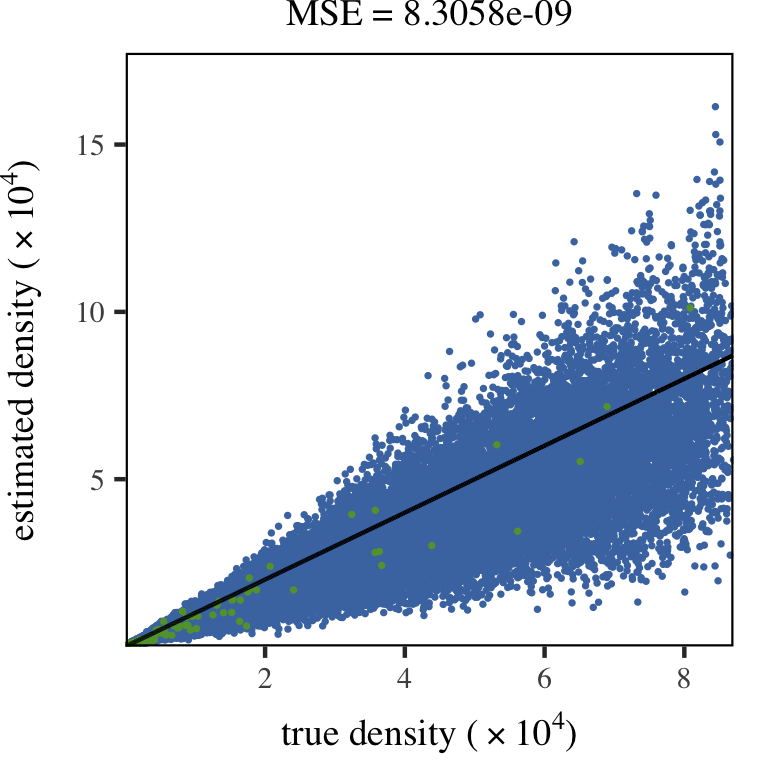
\includegraphics[keepaspectratio=true, width=\textwidth, height=0.23\textheight]{result/img/results_ferdosi_1_60000_mbe_silverman}
	\caption{Set \ferdosiOne, \mbe}
	\label{fig:results:singlesphere:mbe:ferdosi1}
\end{subfigure}
% Ferdosi 1 - SAMBE
\begin{subfigure}{0.3\textwidth}
	\centering
	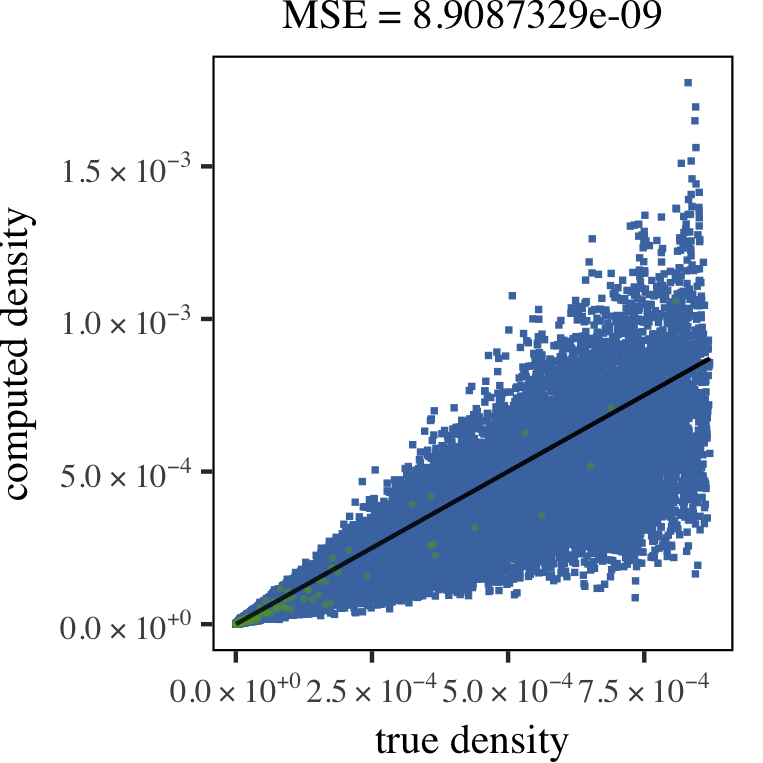
\includegraphics[keepaspectratio=true, width=\textwidth, height=0.23\textheight]{result/img/results_ferdosi_1_60000_sambe_silverman}
	\caption{Set \ferdosiOne, \sambe}
	\label{fig:results:singlesphere:sambe:ferdosi1}
\end{subfigure}
\subfigvspace
% Baakman 1	- MBE
\begin{subfigure}{0.3\textwidth}
	\centering
	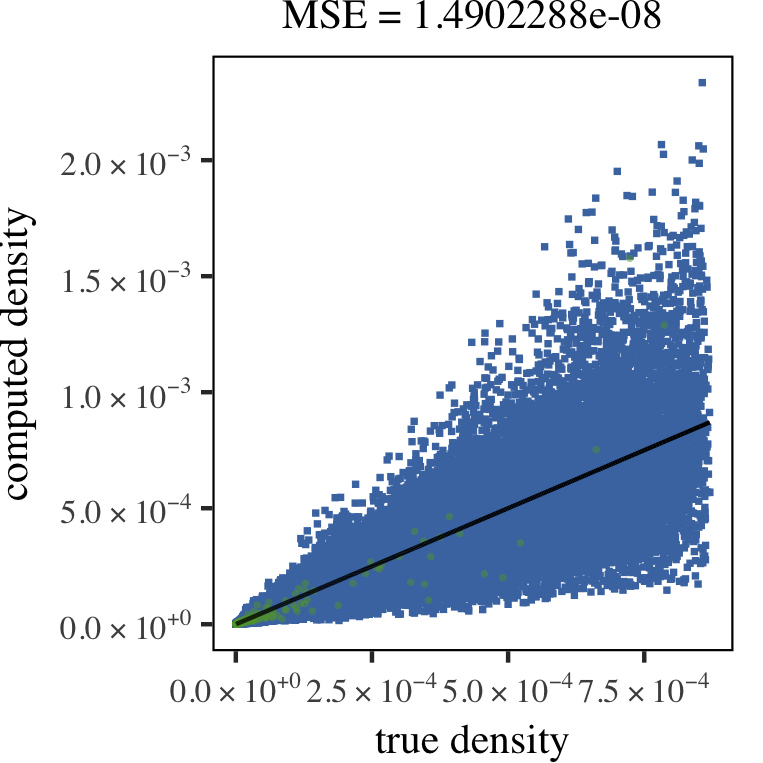
\includegraphics[keepaspectratio=true, width=\textwidth, height=0.23\textheight]{result/img/results_baakman_1_60000_mbe_silverman}
	\caption{Set \baakmanOne, \mbe}
	\label{fig:results:singlesphere:mbe:baakman1}
\end{subfigure}
% Baakman 1	- SAMBE
\begin{subfigure}{0.3\textwidth}
	\centering
	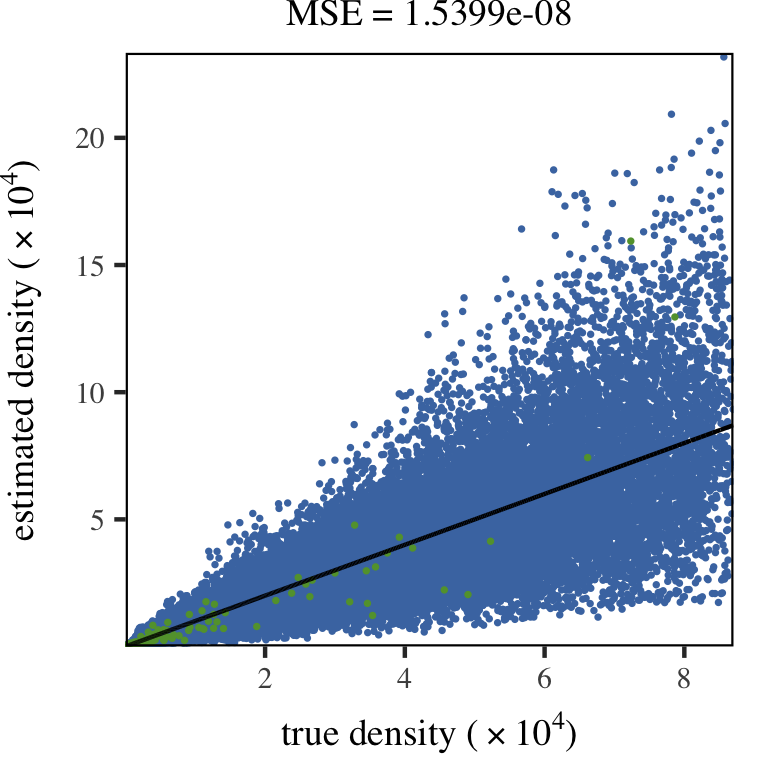
\includegraphics[keepaspectratio=true, width=\textwidth, height=0.23\textheight]{result/img/results_baakman_1_60000_sambe_silverman}
	\caption{Set \baakmanOne, \sambe}
	\label{fig:results:singlesphere:sambe:baakman1}
\end{subfigure}
\subfigvspace
% Baakman 4 - MBE
\begin{subfigure}{0.3\textwidth}
	\centering
	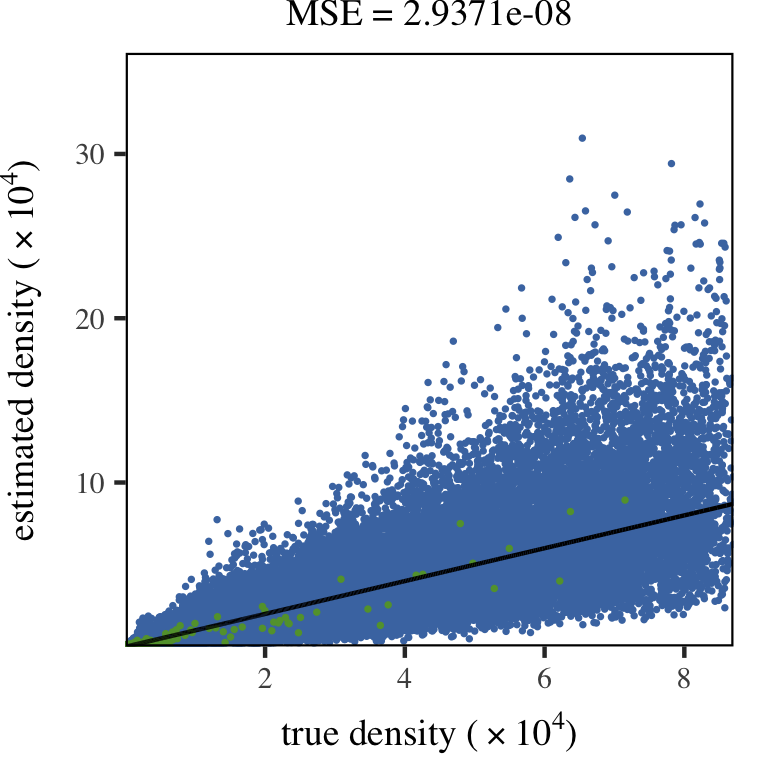
\includegraphics[keepaspectratio=true, width=\textwidth, height=0.23\textheight]{result/img/results_baakman_4_60000_mbe_silverman}
	\caption{Set \baakmanFour, \mbe}
	\label{fig:results:singlesphere:mbe:baakman4}
\end{subfigure}	
% Baakman 4 - SAMBE
\begin{subfigure}{0.3\textwidth}
	\centering
	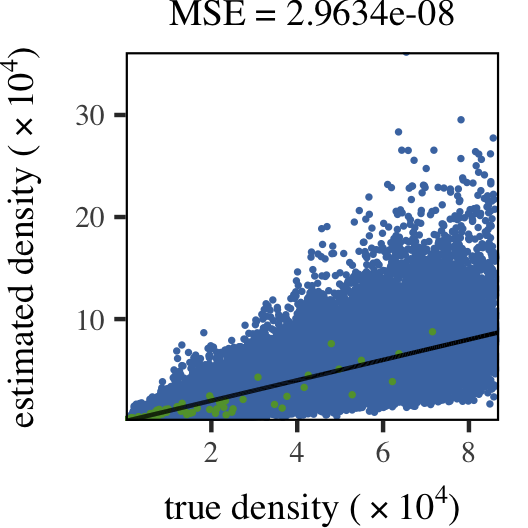
\includegraphics[keepaspectratio=true, width=\textwidth, height=0.23\textheight]{result/img/results_baakman_4_60000_sambe_silverman}
	\caption{Set \baakmanFour, \sambe}
	\label{fig:results:singlesphere:sambe:baakman4}
\end{subfigure}		
\subfigvspace
% Baakman 5 - MBE
\begin{subfigure}{0.3\textwidth}
	\centering
	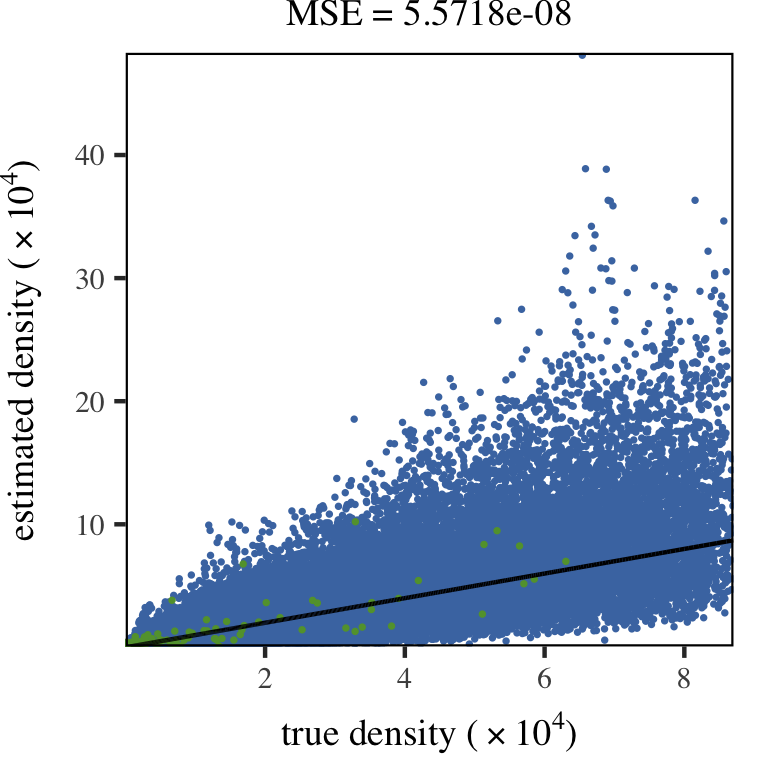
\includegraphics[keepaspectratio=true, width=\textwidth, height=0.23\textheight]{result/img/results_baakman_5_60000_mbe_silverman}
	\caption{Set \baakmanFive, \mbe}
	\label{fig:results:singlesphere:mbe:baakman5}
\end{subfigure}
% Baakman 5 - SAMBE
\begin{subfigure}{0.3\textwidth}
	\centering
	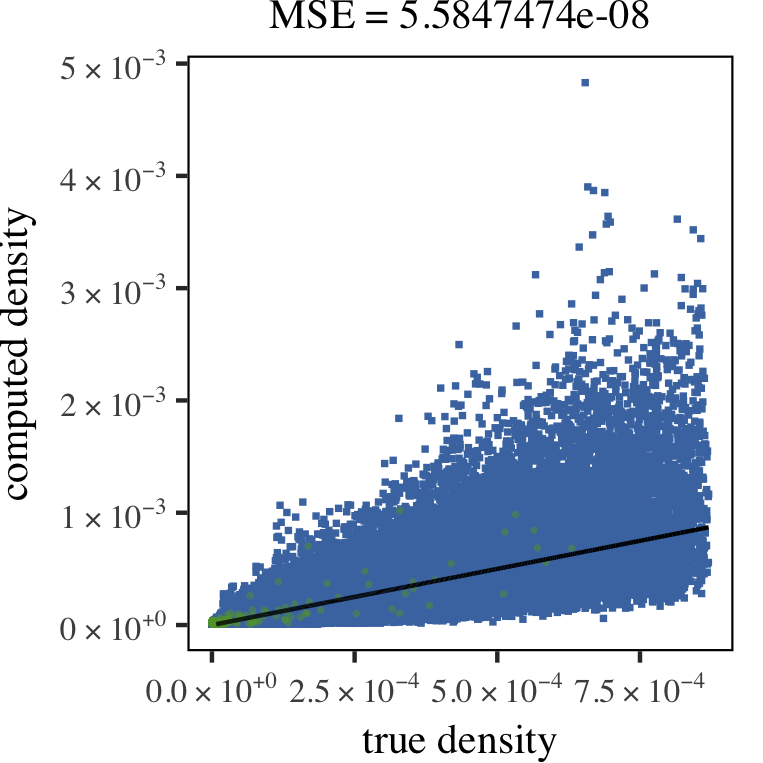
\includegraphics[keepaspectratio=true, width=\textwidth, height=0.23\textheight]{result/img/results_baakman_5_60000_sambe_silverman}
	\caption{Set \baakmanFive, \sambe}
	\label{fig:results:singlesphere:sambe:baakman5}
\end{subfigure}	
		\caption{The density as estimated by \subref{fig:results:singlesphere:mbe:ferdosi1}-\subref{fig:results:singlesphere:mbe:baakman5} \mbe and \subref{fig:results:singlesphere:sambe:ferdosi1}-\subref{fig:results:singlesphere:sambe:baakman5} \sambe as a function of the known density of datasets \ferdosiOne through \baakmanFive.}
		\label{fig:results:singleSphere:comparativePlots}
	\end{figure*}
	%
	This is confirmed by the visualization of the results in \cref{fig:results:singleSphere:comparativePlots} where hardly any difference is visible between \cref{fig:results:singlesphere:mbe:ferdosi1,fig:results:singlesphere:mbe:baakman1,fig:results:singlesphere:mbe:baakman4,fig:results:singlesphere:mbe:baakman5}, and \cref{fig:results:singlesphere:sambe:ferdosi1,fig:results:singlesphere:sambe:baakman1,fig:results:singlesphere:sambe:baakman4,fig:results:singlesphere:sambe:baakman5}, respectively. 
		%Ferdosi 1
		Comparing the plots associated with dataset \ferdosiOne we find that the shape-adaptive estimator tends to overestimate densities more than the symmetric estimator if the Gaussian component is spherical.
		% Baakman 4
		Based on \cref{fig:results:singlesphere:mbe:baakman4,fig:results:singlesphere:sambe:baakman4} the same holds for dataset \baakmanFour. 
	% Focus on components
	Comparing the performance within datasets between the two components showed no marked differences in performance between the estimators between components.

%ANISOTROPY
	\begin{table}
		\centering
		%!TEX root = ../../paper.tex

% \sisetup{
% 	table-format=1.3e+1,
% 	scientific-notation=true, 
% 	table-number-alignment=center,
% }

% Mean and SD in single column
% \begin{tabular}{@{}c*{6}{c}@{}}
% \toprule
% ~				& Full Set 												& \legendComponentOne Gaussian 1						& \legendComponentTwo Gaussian 2						& \legendComponentThree Gaussian 3						& \legendComponentFour Gaussian 4					 	&  \legendComponentNoise Noise\\
% \midrule
% %
% \ferdosiTwo		& \meanSD{1.504005042371507e+00}{5.309582791641542e-01} & \meanSD{1.320121582169093e+00}{1.749869852989719e-01} & \meanSD{1.304784013773833e+00}{1.427734068384871e-01} & ~ 													& ~ 													& \meanSD{1.890276960903559e+00}{7.587403345342156e-01}\\
% \baakmanTwo 	& \meanSD{1.614716145373154e+00}{5.702499690627806e-01} & \meanSD{1.407377455694081e+00}{2.782480127488867e-01} & \meanSD{1.491043432778090e+00}{3.453168397321122e-01}	& ~ 													& ~ 													& \meanSD{11.948464282370670e+00}{7.826307984091438e-01}\\
% \ferdosiThree	& \meanSD{1.460357930082488e+00}{5.507084955708148e-01} & \meanSD{1.294023549845817e+00}{1.889517285607608e-01} & \meanSD{1.265946347671562e+00}{1.301150512342848e-01} & \meanSD{1.291829938425150e+00}{2.103396722315814e-01} & \meanSD{1.275739356043035e+00}{1.654855348814119e-01} & \meanSD{1.819950324176552e+00}{8.111641695146756e-01} \\
% \baakmanThree 	& \meanSD{1.532493079967588e+00}{5.713672219810757e-01} & \meanSD{1.314980484677339e+00}{2.190657831683435e-01} & \meanSD{1.487242917765238e+00}{3.393090417977690e-01} & \meanSD{1.291829938425150e+00}{2.103396722315814e-01} & \meanSD{1.396015162355687e+00}{2.851380764085146e-01} & \meanSD{1.854880861700560e+00}{8.195085323228068e-01}\\
% %
% \bottomrule
% \end{tabular}

\small
\sisetup{
	table-format=1.4,
	scientific-notation=fixed,
	table-number-alignment=center,
	fixed-exponent=0,
	round-mode=figures,
	round-precision=4
}


\begin{tabular}{@{}c*{12}{S}@{}}
\toprule
 				& \multicolumn{2}{c}{~} 						& \multicolumn{2}{c}{\legendComponentOne Gaussian 1} 	& \multicolumn{2}{c}{\legendComponentTwo Gaussian 2}	& \multicolumn{2}{c}{\legendComponentThree Gaussian 3}	& \multicolumn{2}{c}{\legendComponentFour Gaussian 4}	& \multicolumn{2}{c}{\legendComponentNoise Noise} \\
															  	\cmidrule(lr){4-5}							  				\cmidrule(lr){6-7}							  			\cmidrule(lr){8-9} 							  			\cmidrule(lr){10-11} 							  \cmidrule(lr){12-13}
~				& {\mean}				& {\SD}			& {\mean}				 & {\SD}			& {\mean}				 & {\SD}			 & {\mean}				& {\SD}			& {\mean}				& {\SD}			& {\mean}					& {\SD}\\ 			
\midrule
\ferdosiTwo		& 1.504005042371507e+00 & 5.309582791641542e-01 & 1.320121582169093e+00 & 1.749869852989719e-01 & 1.304784013773833e+00 & 1.427734068384871e-01 &  						&  						& 	 					&  							& 1.890276960903559e+00 	& 7.587403345342156e-01\\
\baakmanTwo 	& 1.614716145373154e+00 & 5.702499690627806e-01 & 1.407377455694081e+00 & 2.782480127488867e-01 & 1.491043432778090e+00 & 3.453168397321122e-01 &  						&  						& 	 					&  							& 1.948464282370670e+00 	& 7.826307984091438e-01\\
\ferdosiThree 	& 1.460357930082488e+00 & 5.507084955708148e-01 & 1.294023549845817e+00 & 1.889517285607608e-01 & 1.265946347671562e+00 & 1.301150512342848e-01 & 1.291829938425150e+00 & 2.103396722315814e-01 & 1.275739356043035e+00 & 1.654855348814119e-01 	& 1.819950324176552e+00 	& 8.111641695146756e-01 \\
\baakmanThree 	& 1.532493079967588e+00 & 5.713672219810757e-01 & 1.314980484677339e+00 & 2.190657831683435e-01 & 1.487242917765238e+00 & 3.393090417977690e-01 & 1.291829938425150e+00 & 2.103396722315814e-01 & 1.396015162355687e+00 & 2.851380764085146e-01 	& 1.854880861700560e+00 	& 8.195085323228068e-01\\
\bottomrule
\end{tabular}
		\caption{The mean (\mean) and the standard deviation (\SD) of the anisotropy of the kernels used for the datasets with a single Gaussian.}
		\label{tab:results:singleSphere:anisotropy}
	\end{table}
	%
	% General
	\Cref{tab:results:singleSphere:anisotropy} presents the mean and the standard deviation of the anisotropy of the kernels used for the different datasets. Comparing the means we find a positive correlation between the anisotropy of the Gaussian component of the dataset and mean anisotropy of the kernels. The same positive correlation can be observed for the standard deviation. 
	% Focus on components
	Reviewing these statistics of the components of the datasets reveals that the increase in average anisotropy is primarily caused by an increase in anisotropy op kernels of points sampled from the Gaussian component. The mean anisotropy of the noise component stays relatively constant. Furthermore as the Gaussian component is more anisotropic the variation in anisotropy of the kernels increases.

%Summary
To summarize; in spite of differences in anisotropy of the used kernels we have observed very few differences between two estimators. Using shape-adaptive kernels did not yield the expected gain in performance. We did find the expected influence of the anisotropy of the Gaussian components on the shape of the kernels. 
